\subsubsection{Generation Models}

For a given chess position and a played move, the commentator should create comments on different categories. Those categories are the \textit{description of the current move}, the \textit{description of the move quality}, the \textit{comparison of moves}, the \textit{description of the move planning} and \textit{contextual game information}.\footnote{Cf. \cite{jhamtani-etal-2018-learning}, p. 1663}$^{;}$\footnote{Cf. \cite{zang-etal-2019-automated}, pp. 3-4}

\begin{figure}[h]
\centering
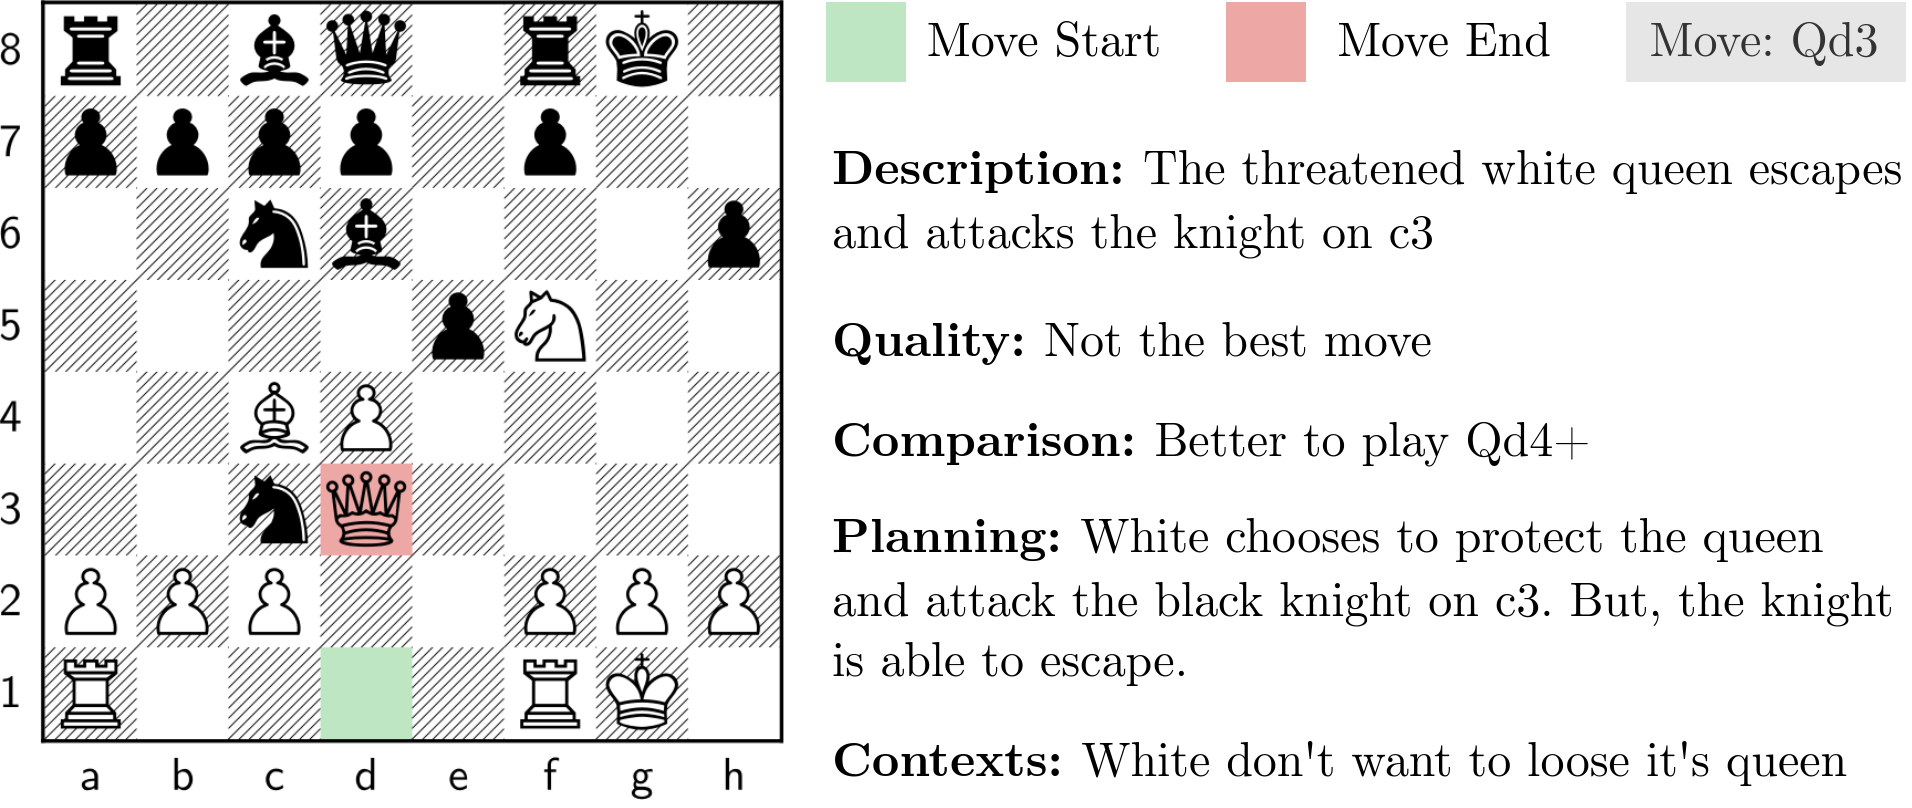
\includegraphics[width=0.7\textwidth]{graphics/commentator_example/commentator.png}
\caption{Chess Commentary Example (Note: Figure based on \cite{zang-etal-2019-automated} Figure 1)}
\end{figure}

Since the procedure for creating comments varies from category to category, it is practically impossible to do this with a single commentator, as simplified described above. Therefore, in the following it will be spoken of five individual ones, each for one of the categories. In addition, instead of categories, it is now spoken of generation models, since these are used to generate comments. These generation models come with two challenges that can have a strong impact on the quality of the generated description: (1) the features on the basis of which the comments for the aspects are generated, (2) the number of moves and the resulting position considered. To overcome the first challenge \cite{jhamtani-etal-2018-learning} used "discrete information (threats, game evaluation scores, etc.)"\footnote{\cite{zang-etal-2019-automated}, p. 4}. How \cite{zang-etal-2019-automated} show, those features information did not provide the best results. Therefore, they have used features provided directly by the internal chess engine. These are the \textit{state of the board before the move}, \textit{start square of the move}, \textit{end square of the move}, \textit{piece on the start square}, \textit{piece on the end square}, \textit{promotion state} and  \textit{checking state}. The pieces on the starting square and on the ending square can be different, since the pawns can be replaced by another piece when they reach the opponent's last rank.\footnote{Cf. \cite{fide-2018-loc} p. 10} In this case the promotion state would be set to 1. The advantage of using these features is that they can be easily read from the information provided by the chess engine described in the previous section. These features can be summarized under the terms position and move, which is why in the following only those two terms are used to described all the features. The second challenge can be overcome by distinguishing between generation models that need only one move (description) and generation models that need multiple moves (comparision, planning and context) so that the description is accurate. Depending on the model, they implement either a single-move encoder (SME) or a multi-move encoder (MME). An execption is the quality model, which doesn't need any move to create description and therefore implements a completly different encoder. These encoders differ in their training so that they can precisely store different amounts of information in the context vector.

The process of encoding and decoding can be represented as a function. $f_{\text{Decode}}$ is the decoder, $f_{\text{SME}}$ the single move encoder, $f_{\text{MME}}$ the multi move encoder and $f_{\text{Encoder}}$ the encoder of the quality model. Encoding and decoding are mapped to an output $C$. This corresponds to the respective comment of a model. This representation helps to understand what information is needed for the translation of the respective translation models. The description model should provide a move explanation for a position $b_0$ and a move $m_0$ played in this position. The process of encoding and decoding can be formulated as $f_{\text{Decoder}}(f_{\text{SME}}(b_0,m_0)) \rightarrow C_{\text{Description}}$\footnote{Cf. \citep{zang-etal-2019-automated}, p.3}. The quality model should describe how good a move was. Therefore it needs three information on basis of which the the commentary is generated. Those are the board before the move, the board after the move and the winning rate difference. For every position evaluated by the chess engines neural network it outputs a value which describes the winning chances of a player (denoted with $v$ in Figure \ref{fig:pae}). The winning rate difference is the difference between the value before and after the move. This can be formulated as $f_{\text{Decoder}}(f_{\text{Encoder}}(b_0,b_1,v_1-v_0)) \rightarrow C_{\text{Quality}}$\footnote{Cf. \citep{zang-etal-2019-automated}, p.4}. The comparision model compares two moves. This requires the move played and the resulting position, as well as a move to compare and it's resulting position. If a player plays a move $m_0$ and it is not the best move, the engine returns the best move $m_1$ for comparison, as well as the resulting positions $b_1$ and $b_2$. If the best move has already been played, the second best move is used for comparison. Since this involves two moves and positions, the multi-move encoder is used. This can be formulated as $f_{\text{Decoder}}(f_{\text{MME}}(b_1,m_0,b_2,m_1)) \rightarrow C_{\text{Comparision}}$\footnote{Cf. \citep{zang-etal-2019-automated}, p.4}. To generate comments for the depth analysis, the planning model receives probable moves played after the current move as well as the resulting positions. $f_{\text{Planning}}(f_{\text{MME}}((b_2,m_1),(b_3,m_2),(b_4,m_3),...)) \rightarrow C_{\text{Planning}}$\footnote{Cf. \citep{zang-etal-2019-automated}, p.4}. Lastly, comments are to be generated for the entire situation. The planning model can simply be extended by the played move, i.e. $f_{\text{Planning}}(f_{\text{MME}}((b_1,m_0),(b_2,m_1),(b_3,m_2),(b_4,m_3),...)) \rightarrow C_{\text{Planning}}$\footnote{Cf. \citep{zang-etal-2019-automated}, p.4}.

Finally, the five generation models still need to be trained. For this purpose, \cite{jhamtani-etal-2018-learning} compiled a dataset of 11,578 annotated chess games, further used by \citep{zang-etal-2019-automated}. they divided the dataset into three sub-datasets for training, validation and testing, in the ratio 7:1:2. In both cases, training with the data set and the generation models described above showed good results.



% With these challenges overcomed the next steps are

% Once these problems are solved, for each requirement, the information needed to fulfill a requirement must be put into a form that can be used as input, certain features can be easily identified, and the text can be generated based on these identifications.

% In order to generate comments on these requirements, it is necessary to define certain features on the basis of which this is done. \cite{jhamtani-etal-2018-learning} uses features such as, \gls{threats} and position value, but as \cite{zang-etal-2019-automated} show, this information does not consider the following positions well enough, which affects the quality of comments. To solve this problem the requirements were divided into two categories: (1) requirements which need exactly one move to be describe, (2) requirements which need a number of moves to be describe. The second category is only an extension of the first, so the two categories differ in detail only in how many positions and moves they consider; the features included remain the same.

% A method which has shown significant success in the field of natural language processing are Recurrent Neural Networks (RNN).

% The process of generating the text commentary can be summarized into two upper parts, namely encoding and decoding. Encoding describes the extraction and formatting of certain features to make them easier to process, while decoding describes the translation of the encoded features into a text format.